% ============================================================
% LLM-BLM 実験 S2：小型株で、決算発表文の読み取りは発表後の変動率（リスク）を予測するか（事前登録した検定の結果）
% コンパイル：tectonic -X compile LLM-BLM_実験S2.tex   （XeTeX 系。このフォルダで実行する）
% 数値と表は 図/values.tex・図/tab_*.tex（作成スクリプト/values.py）、図は 図/*.pdf（作成スクリプト/figs.py）。
% どちらも experiments/S2_smallcap_risk/results から作る。本文に数値を手で書かない。
% ============================================================
\documentclass[xelatex,ja=standard,jafont=haranoaji,a4paper,10pt,openany]{bxjsreport}
\setpagelayout*{left=24mm,right=24mm,top=24mm,bottom=26mm,footskip=11mm}

\usepackage{amsmath,amssymb,mathtools,bm}
\usepackage{booktabs,array,multirow,longtable}
\usepackage{graphicx}
\usepackage{adjustbox}
\usepackage{xcolor}
\usepackage{enumitem}
\usepackage{caption}
\usepackage{float}
\usepackage[most]{tcolorbox}
\usepackage[hidelinks,bookmarksnumbered]{hyperref}

\graphicspath{{図/}}
% values.py が results から作る。手で直さない。
\expandafter\def\csname v@commit\endcsname{ecf16bb}
\expandafter\def\csname v@npanel\endcsname{38,054}
\expandafter\def\csname v@neval\endcsname{15,997}
\expandafter\def\csname v@nevalgpt\endcsname{6,975}
\expandafter\def\csname v@Pcoef\endcsname{$+$1.51}
\expandafter\def\csname v@Punit\endcsname{\%}
\expandafter\def\csname v@Pt\endcsname{$+$4.01}
\expandafter\def\csname v@Pp\endcsname{$<$0.001}
\expandafter\def\csname v@Plo\endcsname{$+$0.77}
\expandafter\def\csname v@Phi\endcsname{$+$2.25}
\expandafter\def\csname v@Pn\endcsname{15,158}
\expandafter\def\csname v@Pdates\endcsname{1,384}
\expandafter\def\csname v@Prtwo\endcsname{0.036}
\expandafter\def\csname v@Pperm\endcsname{0.0010}
\expandafter\def\csname v@Pverdict\endcsname{支持}
\expandafter\def\csname v@Rcoef\endcsname{$+$2.17}
\expandafter\def\csname v@Runit\endcsname{\%}
\expandafter\def\csname v@Rt\endcsname{$+$6.05}
\expandafter\def\csname v@Rp\endcsname{$<$0.001}
\expandafter\def\csname v@Rlo\endcsname{$+$1.47}
\expandafter\def\csname v@Rhi\endcsname{$+$2.88}
\expandafter\def\csname v@Rn\endcsname{13,152}
\expandafter\def\csname v@Rdates\endcsname{1,171}
\expandafter\def\csname v@Rrtwo\endcsname{0.096}
\expandafter\def\csname v@Ncoef\endcsname{$+$1.61}
\expandafter\def\csname v@Nunit\endcsname{\%}
\expandafter\def\csname v@Nt\endcsname{$+$4.25}
\expandafter\def\csname v@Np\endcsname{$<$0.001}
\expandafter\def\csname v@Nlo\endcsname{$+$0.87}
\expandafter\def\csname v@Nhi\endcsname{$+$2.35}
\expandafter\def\csname v@Nn\endcsname{15,158}
\expandafter\def\csname v@Ndates\endcsname{1,384}
\expandafter\def\csname v@Nrtwo\endcsname{0.041}
\expandafter\def\csname v@Fn\endcsname{15,158}
\expandafter\def\csname v@Fbase\endcsname{47.60}
\expandafter\def\csname v@Fwith\endcsname{47.04}
\expandafter\def\csname v@Fgain\endcsname{$-$0.56}
\expandafter\def\csname v@Fratio\endcsname{1.0107}
\expandafter\def\csname v@Ft\endcsname{$-$5.34}
\expandafter\def\csname v@chronomidriskcoefsec\endcsname{$+$1.64}
\expandafter\def\csname v@chronomidrisktsec\endcsname{$+$5.42}
\expandafter\def\csname v@dictuncertaintycoefsec\endcsname{$+$0.37}
\expandafter\def\csname v@dictuncertaintytsec\endcsname{$+$1.51}
\expandafter\def\csname v@dictnegativecoefsec\endcsname{$+$0.94}
\expandafter\def\csname v@dictnegativetsec\endcsname{$+$3.97}
\expandafter\def\csname v@finbertnegativecoefsec\endcsname{$+$0.26}
\expandafter\def\csname v@finbertnegativetsec\endcsname{$+$1.10}
\expandafter\def\csname v@gptflagscoefsec\endcsname{$+$0.56}
\expandafter\def\csname v@gptflagstsec\endcsname{$+$1.85}
\expandafter\def\csname v@gptriskcoefsec\endcsname{$+$1.41}
\expandafter\def\csname v@gptrisktsec\endcsname{$+$4.21}
\expandafter\def\csname v@chronoriskcoefsec\endcsname{$+$1.70}
\expandafter\def\csname v@chronorisktsec\endcsname{$+$3.06}

\newcommand{\V}[1]{\ifcsname v@#1\endcsname\csname v@#1\endcsname\else\textbf{??#1??}\fi}
\newcommand{\tabin}[1]{\adjustbox{max width=\linewidth}{\input{図/tab_#1.tex}}}

\definecolor{c1}{HTML}{2A78D6}
\definecolor{c2}{HTML}{EB6834}
\definecolor{ink2}{HTML}{52514E}
\definecolor{soft1}{HTML}{E4EEF9}
\definecolor{soft2}{HTML}{FBEEDF}

\newcommand{\code}[1]{\texttt{#1}}
\newcommand{\SP}{S\&P500}
\newcommand{\figref}[1]{図~\ref{#1}}
\newcommand{\tabref}[1]{表~\ref{#1}}
\newcommand{\chapref}[1]{第~\ref{#1}~章}

\setlist[itemize]{leftmargin=1.6em,itemsep=0.2em,topsep=0.4em}
\setlist[enumerate]{leftmargin=1.8em,itemsep=0.2em,topsep=0.4em}
\captionsetup{font=small,labelfont=bf,skip=6pt}
\renewcommand{\arraystretch}{1.2}

\makeatletter
\def\@makechapterhead#1{\vspace*{0.3\Cvs}{\parindent\z@\raggedright\normalfont
  \ifnum\c@secnumdepth>\m@ne\if@mainmatter{\Large\headfont\@chapapp\thechapter\@chappos}\par\nobreak\vskip0.4\Cvs\fi\fi
  \interlinepenalty\@M\LARGE\headfont #1\par\nobreak\vskip 1.5\Cvs}}
\def\@makeschapterhead#1{\vspace*{0.3\Cvs}{\parindent\z@\raggedright\normalfont
  \interlinepenalty\@M\LARGE\headfont #1\par\nobreak\vskip 1.5\Cvs}}
\makeatother

\newtcolorbox{keybox}[1][要点]{enhanced,breakable,colback=soft1,colframe=c1,boxrule=0.5pt,arc=2pt,
  left=8pt,right=8pt,top=6pt,bottom=6pt,title={#1},fonttitle=\sffamily\bfseries\small,coltitle=white}
\newtcolorbox{notebox}[1][注意]{enhanced,breakable,colback=soft2,colframe=c2,boxrule=0.5pt,arc=2pt,
  left=8pt,right=8pt,top=6pt,bottom=6pt,title={#1},fonttitle=\sffamily\bfseries\small,coltitle=white}

\title{LLM-BLM 実験 S2\\[6pt]
  \large 小型株で、決算発表文の読み取りは\\発表後の変動率（リスク）を予測するか}
\author{実験の報告書（事前登録した検定の結果）}
\date{2026 年 10 月 24 日}

\begin{document}
\maketitle

\chapter*{概要}
\addcontentsline{toc}{chapter}{概要}

実験 S1 では、小型株で、決算発表文の読み取りが発表後のドリフト（リターンの向き）を予測した。この実験 S2 では、同じ 1,000 社の決算発表文で、読み取りが発表後の\textbf{変動率（リスク）}を、過去の変動率を超えて予測するかを、事前登録して 1 回だけ確かめた。

\begin{keybox}[要点]
\begin{itemize}
\item \textbf{主な検定は支持された}。ChronoGPT（2015 年版）のベクトルに、変動率の驚きを正解にしたリッジを当てた点数が 1 標準偏差高い発表は、発表の前の変動率・2 日の反応の大きさなどを統制した後、2〜60 取引日の変動率が \V{Pcoef}\V{Punit} 高かった（$t$ = \V{Pt}、置換の片側 $p$ \V{Pperm}、発表 \V{Pn} 件）。2021 年以降では \V{Rcoef}\V{Runit}（$t$ = \V{Rt}）。
\item \textbf{ただし大きさは小さい}。決定係数の増分は \V{Prtwo} ポイントで、変動率の大部分は発表の前の変動率で説明される。
\item \textbf{ほかの点数}：ChronoGPT の 26 層目、gpt-4o-mini の 14 項目＋リッジ、辞書の否定的な語も有意に正。辞書の不確実さの語、FinBERT の否定的な文は有意でなかった。2 日の反応の大きさは、辞書の否定的な語や gpt-4o-mini のリスクの印の数がよく予測した。
\item \textbf{標本外の予測には役立たなかった}。四半期ごとに学習した単純な予測のモデルに点数を足すと、二乗誤差はわずかに大きくなった（比 \V{Fratio}、$t$ = \V{Ft}）。点数の情報は、同じ時期の銘柄どうしの相対的なリスクについてのもので、変動率の水準の予測には効かなかった。
\item \textbf{次}：BLM の $\Omega$ や量の調整に、リスクの点数を相対的に使う（新しい事前登録の追記として）。
\end{itemize}
\end{keybox}


\setcounter{tocdepth}{1}
{\small\tableofcontents}

% ============================================================
\chapter{目的}\label{ch:purpose}

実験 S1 では、小型株で、ChronoGPT＋リッジの決算発表文の読み取りが、発表後 2〜60 日のドリフト（リターンの向き）を予測した。しかし、規模で加重した月次のポートフォリオでは、有意な差にならなかった。

リターンの平均より、変動率（リスク）のほうが予測しやすい。変動率には強い持続性があり、過去の変動率でかなり説明できる。文章の不確実さや否定的な語が、その後の変動率と関係するという研究もある。そこで、次の問いを確かめた。

\begin{keybox}[問い]
決算発表文の読み取りは、過去の変動率と 2 日の反応の大きさを超えて、発表後 2〜60 取引日の変動率を予測するか。
\end{keybox}

予測できれば、BLM の見通しの不確かさ（$\Omega$）や量の調整に使える。この実験では、その応用は検定しない。

% ============================================================
\chapter{事前登録}\label{ch:prereg}

検定の仮説・データ・変数・方法・判定の基準は \code{experiments/S2\_smallcap\_risk/preregistration.md} に書き、実行するコード（\code{run.py}）と同じコミットで固定してから、1 回だけ実行した。実行に使ったコミットは \code{\V{commit}}（\code{results/summary.json} に記録）。

\begin{itemize}
\item \textbf{書いた時点で見ていたもの}：S1 のすべての結果（点数と符号つきの超過リターンの関係）。
\item \textbf{見ていなかったもの}：どの銘柄の、どの期間の変動率も計算していなかった。点数と変動率、点数と反応の大きさ（絶対値）の関係も、一度も計算していなかった。
\item \textbf{主な検定 P}：2020 年以降・範囲の中の発表で、\code{log\_rv\_2\_60} を \code{chrono\_risk} と統制・固定効果で回帰した係数が正か。
\item \textbf{判定}：片側 $t$ の $p < 0.05$、かつ、同じ反応日の中で点数を 1,000 回入れ替える置換の片側 $p < 0.05$ なら「支持」。
\item \textbf{副次}（判定に使わない）：ほかの点数（2 つの族でそれぞれ Holm）、2 つの期間 × 4 つの目的変数の比較の表、標本外の予測の比較、2021 年以降と 2 日の反応の大きさを統制から外した頑健性。
\end{itemize}

% ============================================================
\chapter{データと変数}\label{ch:data}

\section{標本}

S1 と同じ 1,000 社（今も上場している会社）の決算発表文。2015 年以降の発表は \V{npanel} 件、評価する発表（2020 年以降、提出日に範囲の中）は \V{neval} 件、gpt-4o-mini の点数がそろう 2024 年以降の発表は \V{nevalgpt} 件。2015〜2019 年の発表は学習にだけ使った。

\section{目的変数}

反応日を day 0 として、調整後終値の日次の対数リターンから計算した（年率、$\sqrt{252}$ 倍）。

\begin{itemize}
\item 主：\code{log\_rv\_2\_60}：2〜60 取引日目の変動率の対数（59 日のうち 40 日以上のリターンがあるもの）
\item 副：\code{log\_rv\_2\_21}（2〜21 日目）、\code{log\_ivol\_2\_60}（IWM との日次の差の変動率、2〜60 日目）、\code{abs\_r\_0\_1}（2 日の反応の大きさ $|$\code{abn\_r\_0\_1}$|$）
\end{itemize}

係数は、点数が 1 標準偏差高いときの差で、対数の変動率では「\%」（対数の差 × 100、ほぼ変動率の比の \%）、反応の大きさでは「bp」で示す。

\section{統制}

発表の前の変動率（\code{log\_rv\_pre}：$-60$〜$-1$ 日、\code{log\_rv\_long}：$-252$〜$-61$ 日）、規模（\code{log\_float}）、決算と売上の驚きの大きさ（$|$SUE$|$、$|$売上の驚き$|$、欠けの印）、業種と年・四半期の固定効果。2 日の反応の大きさ（day 1 の終値で分かる）も統制に入れた（目的変数が反応の大きさのときは除く）。標準誤差は反応日ごとにまとめた。

\section{点数}

\begin{table}[H]
\centering\small
\caption{比べた点数（どれも「高いほどリスクが高い」向き。評価する標本の中で標準化）}
\label{tab:scores}
\begin{tabular}{@{}lp{0.6\linewidth}l@{}}
\toprule
列 & 中身 & 学習 \\
\midrule
\code{chrono\_risk} & ChronoGPT 2015 年版、元の文章の最後の層の平均（S1 と同じベクトル）に、四半期ごとのリッジ（主） & 変動率の驚き \\
\code{chrono\_mid\_risk} & ChronoGPT 2015 年版、掃除した文章の 26 層目の平均に、同じリッジ & 変動率の驚き \\
\code{dict\_uncertainty} & Loughran--McDonald の不確実さの語の割合 & なし \\
\code{dict\_negative} & Loughran--McDonald の否定的な語の割合 & なし \\
\code{finbert\_negative} & FinBERT の否定的な文の割合 & なし \\
\code{gpt\_flags} & gpt-4o-mini のリスクの印 10 個の数 & なし \\
\code{gpt\_risk} & gpt-4o-mini の 14 の項目に、同じリッジ & 変動率の驚き \\
\bottomrule
\end{tabular}
\end{table}

学習ありの点数の正解は「変動率の驚き」$\log(\mathrm{rv}_{2\text{〜}60} / \mathrm{rv}_{\text{pre}})$ で、その四半期が始まる前に 60 日の窓が閉じた発表だけで学習した。

% ============================================================
% 結果の章（数値は 図/values.tex と 図/tab_*.tex から。手で書かない）

% ============================================================
\chapter{主な検定}\label{ch:primary}

\begin{table}[H]
\centering\small
\caption{主な検定 P：2020 年以降・範囲の中の発表で、2〜60 取引日の変動率（対数）を \code{chrono\_risk} と統制・固定効果で回帰した結果}
\label{tab:primary}
\begin{tabular}{@{}lr@{}}
\toprule
点数が 1 標準偏差高いときの変動率の差 & \V{Pcoef}\V{Punit} \\
95\% 信頼区間 & [\V{Plo}, \V{Phi}]\V{Punit} \\
$t$（反応日ごとにまとめた標準誤差） & \V{Pt} \\
片側 $p$ & \V{Pp} \\
置換（同じ反応日の中で 1,000 回）の片側 $p$ & \V{Pperm} \\
発表の数（反応日の数） & \V{Pn}（\V{Pdates}） \\
決定係数の増分 & \V{Prtwo} ポイント \\
\midrule
判定 & \textbf{\V{Pverdict}} \\
\bottomrule
\end{tabular}
\end{table}

\begin{keybox}[結果]
事前登録の判定の基準を両方とも満たし、仮説は\textbf{支持}された。ChronoGPT＋リッジの点数が 1 標準偏差高い発表は、発表の前の変動率（2 つの期間）・2 日の反応の大きさ・規模・驚きの大きさ・業種と時期の固定効果を統制したうえで、その後 2〜60 取引日の変動率が \V{Pcoef}\V{Punit} 高かった。1,000 回の置換のどれも、実際の係数を超えなかった。
\end{keybox}

\begin{itemize}
\item \textbf{大きさは小さい}：1 標準偏差で約 1.5\%（変動率の比で、例えば年 50\% が 50.8\% になる程度）。決定係数の増分は \V{Prtwo} ポイントで、変動率のばらつきの大部分は、発表の前の変動率で説明される。
\item \textbf{2021 年以降}：\V{Rcoef}\V{Runit}（$t$ = \V{Rt}）。同じ向きで、より大きい。
\item \textbf{2 日の反応の大きさを統制から外す}：\V{Ncoef}\V{Nunit}（$t$ = \V{Nt}）。ほとんど変わらない。点数の情報は、市場が 2 日で示した反応の大きさとは別のものである。
\end{itemize}

% ============================================================
\chapter{副次の検定と比較}\label{ch:secondary}

\section{ほかの点数}

\begin{table}[H]
\centering\small
\caption{副次の検定：2〜60 日の変動率の回帰（係数は変動率の \%。族ごとに Holm の補正）}
\label{tab:secondary}
\tabin{secondary}
\end{table}

\begin{itemize}
\item \textbf{ChronoGPT の 26 層目}（掃除した文章）は、主のモデルと同じくらい強く、Holm の補正の後も有意だった。
\item \textbf{学習なしの点数}：辞書の否定的な語の割合は有意に正（\V{dictnegativecoefsec}\%、$t$ = \V{dictnegativetsec}）だった。辞書の不確実さの語と、FinBERT の否定的な文の割合は、有意でなかった。「不確実さ」の語が変動率を予測するという直感とは違う結果である。
\item \textbf{gpt-4o-mini の期間}（2024 年以降）：14 の項目に重みを学習したもの（\V{gptriskcoefsec}\%、$t$ = \V{gptrisktsec}）と、ChronoGPT＋リッジ（\V{chronoriskcoefsec}\%、$t$ = \V{chronorisktsec}）が強く、リスクの印の数（学習なし）は弱かった（\V{gptflagscoefsec}\%、$t$ = \V{gptflagstsec}。Holm の補正の後も 5\% で有意）。
\end{itemize}

\section{比較の表}

\begin{table}[H]
\centering\small
\caption{2020 年以降：係数と、括弧の中は $t$}
\label{tab:compare2020}
\tabin{compare_2020}
\end{table}

\begin{table}[H]
\centering\small
\caption{2024 年以降（gpt-4o-mini の点数がそろう発表）：係数と、括弧の中は $t$}
\label{tab:compare2024}
\tabin{compare_2024}
\end{table}

\begin{figure}[H]
\centering
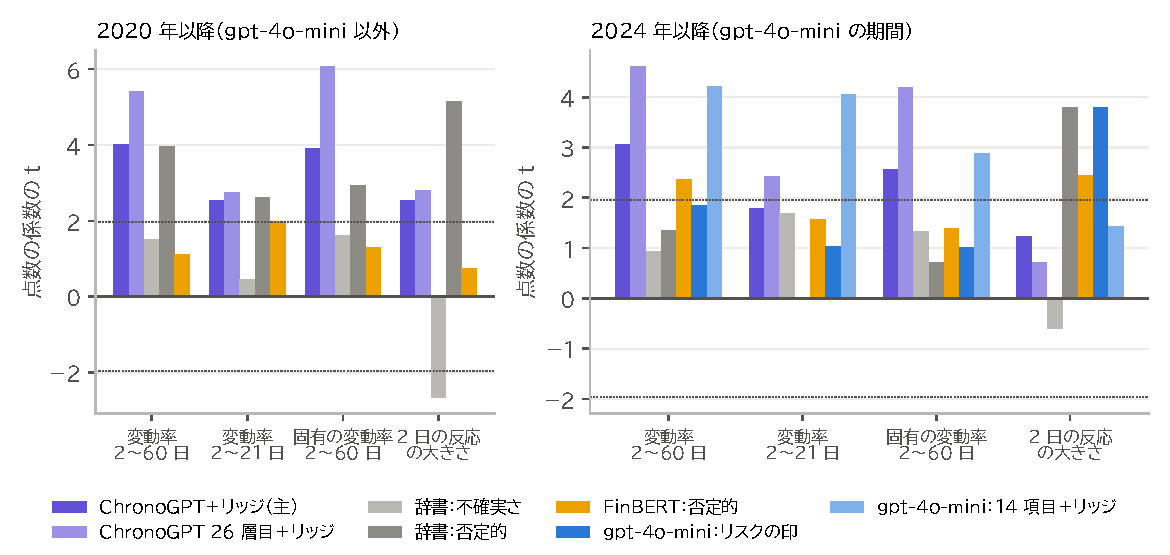
\includegraphics[width=\linewidth]{compare.pdf}
\caption{点数の係数の $t$。点線は $\pm 1.96$。}
\label{fig:compare}
\end{figure}

\begin{itemize}
\item 学習ありの点数（ChronoGPT の 2 つ、gpt-4o-mini の 14 項目）は、2〜60 日・2〜21 日・固有の変動率のどれでも正だった。
\item \textbf{2 日の反応の大きさ}は、学習なしの点数のほうがよく説明した。辞書の否定的な語、gpt-4o-mini のリスクの印の数、FinBERT の否定的な文（2024 年以降）は、反応が大きくなることを予測した。一方、辞書の不確実さの語は、2020 年以降では反応が\textbf{小さい}ことと関係した。悪い知らせを多く含む発表ほど、株価が大きく動く。
\end{itemize}

% ============================================================
\chapter{標本外の予測}\label{ch:forecast}

事前登録の副次の 4：2020 年以降の各四半期について、その四半期の前に 60 日の窓が閉じた発表だけで最小二乗を学習し、2〜60 日の変動率（対数）を予測した。基準のモデル（発表の前の変動率、規模、2 日の反応の大きさ、驚きの大きさ）と、それに ChronoGPT＋リッジの点数を足したモデルを比べた。

\begin{table}[H]
\centering\small
\caption{標本外の予測の比較（発表 \V{Fn} 件）}
\label{tab:forecast}
\begin{tabular}{@{}lr@{}}
\toprule
標本外の決定係数（基準のモデル） & \V{Fbase}\% \\
標本外の決定係数（基準＋点数） & \V{Fwith}\% \\
差 & \V{Fgain} ポイント \\
二乗誤差の比（＋点数 ÷ 基準） & \V{Fratio} \\
損失の差（基準 − ＋点数）の平均の $t$ & \V{Ft} \\
\bottomrule
\end{tabular}
\end{table}

\begin{figure}[H]
\centering
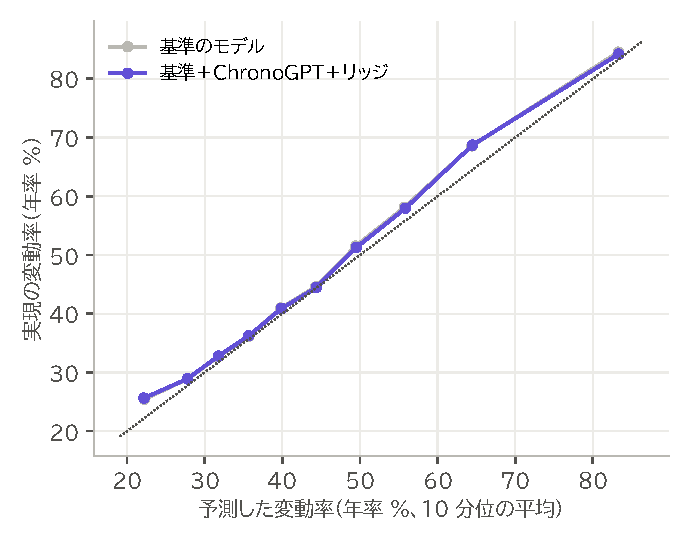
\includegraphics[width=0.6\linewidth]{forecast.pdf}
\caption{予測した変動率と実現の変動率（予測の 10 分位ごとの平均）。2 本の線はほぼ重なる。点線は予測＝実現。}
\label{fig:forecast}
\end{figure}

\begin{keybox}[結果]
発表の前の変動率などの基準のモデルだけで、標本外の決定係数は \V{Fbase}\% あった。そこに点数を足すと、予測は\textbf{わずかに悪くなった}（二乗誤差の比 \V{Fratio}、$t$ = \V{Ft}）。回帰の検定（\chapref{ch:primary}）で見えた情報は、この単純な水準の予測では役に立たなかった。
\end{keybox}

\subsection*{年ごとの内訳（実行の後に加えた記述）}

\begin{table}[H]
\centering\small
\caption{標本外の予測の二乗誤差の年ごとの平均（事前登録にない記述）}
\label{tab:forecastyear}
\tabin{forecast_year}
\end{table}

悪化は主に 2021 年に生じ、ほかの年はほぼ同じだった。2020 年は、新型コロナの急落で市場全体の変動率が予想より大きく、どちらのモデルも大きく外した（平均の誤差が大きい）。この予測のモデルは、時期の固定効果を持たないので、市場全体の変動率の水準の変化をそのまま誤差として受ける。

% ============================================================
\chapter{解釈}\label{ch:interpret}

\section{何が分かったか}

\begin{enumerate}
\item \textbf{決算発表文の読み取りは、その後の変動率を予測した}。過去の変動率と 2 日の反応の大きさを統制しても残り、置換の検定でも偶然では説明できない。2021 年以降ではより強い。
\item \textbf{ただし大きさは小さい}。1 標準偏差で変動率が約 1.5\% 高くなる程度で、変動率のばらつきの大部分は、発表の前の変動率で説明される（ヘッジファンドの報告書の第 8 章：変動率は持続性が強い）。
\item \textbf{学習ありの読み取りが効いた}。ChronoGPT のベクトルや gpt-4o-mini の 14 の項目に、変動率の驚きを正解にして重みを学習したものが強く、学習なしの点数では、辞書の否定的な語だけが効いた。
\item \textbf{水準の予測には役立たなかった}。四半期ごとに学習した単純な予測のモデルでは、点数を足すと予測がわずかに悪くなった。回帰の検定は同じ時期の銘柄どうしを比べる（時期の固定効果）のに対し、予測のモデルは水準を当てる必要があり、市場全体の変動率の変化に誤差の大部分が支配される。また、点数は四半期ごとに学習し直すリッジの出力なので、その尺度が時期によって変わる可能性がある。
\end{enumerate}

\section{BLM への使い道}

点数の情報は「同じ時期の銘柄どうしの相対的なリスク」についてのものである。BLM に使うなら、変動率の水準を置き換えるのではなく、次のような相対的な使い方が筋がよい（次の事前登録の追記の候補）。

\begin{itemize}
\item 見通しの不確かさ $\Omega$ を、リスクの点数の順位に応じて銘柄ごとに大きく・小さくする。
\item 共分散の対角（固有の分散）を、点数の順位で少しだけ補正する。
\item 発表の後、リスクの点数の高い銘柄の量を抑える。
\end{itemize}

\section{注意すべき点}

\begin{itemize}
\item 標本は今も上場している会社だけで、変動率の高い時期に消えた会社が抜けている可能性がある。
\item 変動率は日次の終値で測った。日中のデータがあれば、より正確に測れる。
\item gpt-4o-mini の期間は短い。
\item 1 回の実行の結果である。
\end{itemize}


% ============================================================
\chapter{限界}\label{ch:limits}

\begin{itemize}
\item \textbf{生き残った会社だけ}：上場をやめた会社は、変動率の高い時期に消えやすいので、高い変動率の発表が欠けている可能性がある。
\item \textbf{日次の終値だけ}：日中のデータはないので、実現の変動率は日次の終値で測った。
\item \textbf{gpt-4o-mini の期間}は短く、\code{gpt\_risk} は 60 日の窓が閉じるまで学習できないので、さらに短い。
\item \textbf{応用は未検定}：予測した変動率を BLM の $\Omega$ や量の調整に使う効果は、この実験では確かめていない。
\item \textbf{1 回の結果}：事前登録の通り 1 回だけ実行した。
\end{itemize}

% ============================================================
\chapter*{再現の手順}
\addcontentsline{toc}{chapter}{再現の手順}

リポジトリの直下で（\code{.venv} の Python）：

\begin{enumerate}
\item データと点数：S1 と同じ（\code{smallcap.build}、\code{smallcap.score}）。
\item 検定：\code{python experiments/S2\_smallcap\_risk/run.py}（結果は \code{results/}。2 回目は summary.json があると止まる）。
\item この報告書の数値・表と図：\code{資料集/02\_実験/実験S2\_小型株のリスク予測/作成スクリプト/} の \code{values.py} と \code{figs.py}。
\item コンパイル：このフォルダで \code{tectonic -X compile LLM-BLM\_実験S2.tex}。
\end{enumerate}

\end{document}
